\documentclass[9pt]{beamer}

%%pacotes referentes ao Beamer
%\useoutertheme{split}
%\setbeamertemplate{navigation symbols}{}

%\usetheme{beamertheme}
%\usebeamercolor{beamer-color name}

%\usetheme{Boadilla}
%\usecolortheme{dove}

\usetheme{CambridgeUS}
\usecolortheme{beaver}

% \usetheme{pittsburgh}
% \usecolortheme{dolphin}
%\usecolortheme{dove}
%\usecolortheme{seahorse}

%\usetheme{Montpellier}

%number in figures an tables -- beamer
\setbeamertemplate{caption}[numbered]

%Colocar no description
%[leftmargin=!,labelwidth=\widthof{Turma A}]
	
%pacotes usuais do latex
\usepackage[portuguese]{babel}
\usepackage[utf8]{inputenc}
\usepackage{bm}
\usepackage{graphicx}
\usepackage{subfigure}
\usepackage[round]{natbib}
\usepackage{tikz}
\usetikzlibrary{shapes,arrows}
\usepackage{natbib}
\usepackage{times}
\usepackage{calc} %computes the length of a string
\usepackage{dsfont} %pacote para o 1 estilisado para indicadora
\usepackage{enumerate} %permite fazer uns enumerates diferentes
\usepackage[font=small,labelfont=bf]{caption} %permite colocar um segundo caption
\usepackage{booktabs} % comando \toprule, \midrule e \bottomrule
\usepackage{times} %times new roman font
\usepackage{multirow} %comando \multirow
\usepackage{setspace}
\usepackage{xcolor} %texto colorido
\usepackage{booktabs} %costumized tabs
\usepackage{tikz}
\usepackage{hyperref}

\usetikzlibrary{decorations.pathreplacing}

%código para alinhar a esquerda os itens no description
\defbeamertemplate{description item}{align left}{\insertdescriptionitem\hfill}
\defbeamertemplate{enumerate item}{align left}{\insertdescriptionitem\hfill}



%AMS packages
\usepackage{amsmath}
\usepackage{amsfonts}
\usepackage{amssymb}

%Não quebre linhas
\binoppenalty=\maxdimen
\relpenalty=\maxdimen

%Comandos criados por mim
\DeclareMathOperator*{\argmin}{arg\,min}

\DeclareMathOperator*{\argmax}{arg\,max}


\DeclareMathOperator{\espe}{E}

\DeclareMathOperator{\spann}{span}

\DeclareMathOperator{\cov}{Cov}

\DeclareMathOperator{\vari}{Var}

%Informações para o primeiro slide
\date{}
\title[Estatística Básica]{Conceitos básicos}
\author[Gilberto Sassi]{Gilberto Pereira Sassi}
\institute[IME -- UFBA]{Universidade Federal da Bahia \\ Instituto de Matem\'{a}tica e Estat\'{i}stica\\ Departamento de Estat\'{i}stica }

\begin{document}
	
\tikzstyle{decision} = [diamond, draw, fill=blue!20, 
text width=4.5em, text badly centered, node distance=3cm, inner sep=0pt]
\tikzstyle{block} = [rectangle, draw, fill=blue!20, 
text width=5em, text centered, rounded corners, minimum height=4em]
\tikzstyle{line} = [draw, -latex]
\tikzstyle{cloud} = [draw, ellipse,fill=red!20, node distance=3cm,
minimum height=2em]
	
%Slide inicial
\begin{frame}{}
	\maketitle
\end{frame}

%primeiro slide
\section{Programa de curso}
\begin{frame}{Programa do curso}
 \begin{enumerate}
 {\small
  \item Estatística descritiva: tabela de distribuição de frequência e gráficos (gráfico de barras e histograma), associação entre variáveis;
  \item Medidas de resumo: medidas de posição e medidas de dispersão;
  \item Probabilidade: axiomas de probabilidade, espaço amostral, ponto amostral;
  \item Probabilidade condicional: regra de produto das probabilidades, teorema de probabilidade total e teorema de Bayes;
  \item Variável aleatória discreta: valor esperado e variância;
  \item Modelos probabilísticos para variável aleatória discreta: Uniforme, Bernoulli, Binomial, Poison, Geométrico;
  \item Variável aleatória contínua: valor esperado e variância;
  \item Modelos probabilísticos: Uniforme, Normal, Exponencial, t-Student, Qui-quadrado;
  \item Distribuições amostrais e teorema do limite central;
  \item Estimativa intervalar: média e proporção;
  \item Teste de Hipóteses: Erros tipo I e II, nível de significância, poder do teste;
  \item Teste para média e proporção;
  \item p-valor;
  \item Teste de aderência: qui-quadrado;
  \item Associação entre duas variáveis quantitativas: gráfico de dispersão e coeficiente de correlação linear de Pearson;
  \item Regressão linear simples;
  \item Qualidade do ajuste: análise de resíduo.
  }
 \end{enumerate}
\end{frame}


% slide 2
\section{Critério de avaliação, referências e contato}
\begin{frame}{Critério de avaliação}
\begin{block}{Critério de avaliação}
  \begin{itemize}
  \item Duas provas: $P_1$ e $P_2$;
  \item Nota final: $NF = \dfrac{P_1+P_2}{2}$.
 \end{itemize}
\end{block}

\vfill

\begin{block}{Datas de provas}
 \begin{itemize}
  \item Primeira prova: 28/04/2020;
  \item Segunda prova: 30/06/2020;
  \item Segunda chamada da primeira prova:07/07/2020;
  \item Segunda chamada da segunda prova: 09/07/2020.
 \end{itemize}
\end{block} 

\vfill

\begin{block}{Página: listas e slides do curso}
 \url{https://gilberto-sassi.github.io}
\end{block}


\end{frame}


\begin{frame}{Referências}
\textbf{Principal}
 \begin{enumerate}
  \item Barbetta, Pedro Alberto -- Estatística Aplicada às Ciências Sociais;
  \item Bussab, Wilton de Oliveira; Morettin, Pedro Alberto -- Estatística Básica;
 \end{enumerate}

 \vfill
 
\textbf{Complementar}
 \begin{enumerate}
  \item Soares, José Francisco; Siqueira, Armindo Lúcia -- Introdução a estatística médica;
  \item Triola, Mario F. -- Introdução a estatística.
 \end{enumerate}
\end{frame}

\begin{frame}{Contato}

  \begin{block}{E-mail}
   \href{mailto:gilberto.sassi@ufba.br}{gilberto.sassi@ufba.br}
 \end{block}

 \vfill
 
 \begin{block}{Onde me encontrar}
  Sala 220 do Instituto de Matemática e Estatística.
 \end{block}
\end{frame}

\section{Estatística descritiva}
\begin{frame}{Tipos de inferência}
%  De um modo geral, podemos afirmar que a essência da ciência é inferir e existem dois tipos de inferência: dedutiva e indutiva.
 
 \vfill
 
 \begin{block}{Dedutiva}
  Usa-se argumentos lógicos para chegar a conclusões a partir de premissas.

  \textbf{Exemplo}: 
  \begin{itemize}
   \item Premissa: Todo ser humano nascido em solo brasileiro, tem direito a cidadania brasileira. 
   \item João nasceu em Salvador, então João tem direito a cidadania brasileira.
  \end{itemize}
 \end{block}

 \vfill
 
 \begin{block}{Indutiva}
  Processo de generalização da parte ao todo. (Objeto de estudo desse curso). 
  
  \textbf{Exemplo}: Em uma pesquisa eleitoral, entrevista-se parte do eleitorado para estudar a intenção de votos para cada candidato.
  \begin{figure}
   \centering
   \begin{tikzpicture}[scale = 0.2]
   \filldraw[blue!30] (0,0) circle (3);
   \draw[blue] (0,0) circle (3);
   \draw (0,0) circle (6);
   \filldraw[black] (0,0) circle (0.2);
   \filldraw[black] (0,1) circle (0.2);
   \filldraw[black] (0,2) circle (0.2);
   \filldraw[black] (1,0) circle (0.2);
   \filldraw[black] (2,0) circle (0.2);
   \filldraw[black] (-1,0) circle (0.2);
   \filldraw[black] (-2,0) circle (0.2);
   \filldraw[black] (0,-1) circle (0.2);
   \filldraw[black] (0,-2) circle (0.2);
   \filldraw[black] (1,1) circle (0.2);
   \filldraw[black] (1,2) circle (0.2);
   \filldraw[black] (2,1) circle (0.2);
   \filldraw[black] (-1,1) circle (0.2);
   \filldraw[black] (-1,2) circle (0.2);
   \filldraw[black] (-2,1) circle (0.2);
   \filldraw[black] (-1,-1) circle (0.2);
   \filldraw[black] (-1,-2) circle (0.2);
   \filldraw[black] (-2,-1) circle (0.2);
   \filldraw[black] (1,-1) circle (0.2);
   \filldraw[black] (1,-2) circle (0.2);
   \filldraw[black] (2,-1) circle (0.2);
   \filldraw[black] (0,4) circle (0.2);
   \filldraw[black] (0,5) circle (0.2);
   \filldraw[black] (1,4) circle (0.2);
   \filldraw[black] (1,5) circle (0.2);
   \filldraw[black] (2,3) circle (0.2);
   \filldraw[black] (2,4) circle (0.2);
   \filldraw[black] (2,5) circle (0.2);
   \filldraw[black] (3,2) circle (0.2);
   \filldraw[black] (3,3) circle (0.2);
   \filldraw[black] (3,4) circle (0.2);
   \filldraw[black] (4,1) circle (0.2);
   \filldraw[black] (4,2) circle (0.2);
   \filldraw[black] (4,3) circle (0.2);
   \filldraw[black] (5,1) circle (0.2);
   \filldraw[black] (5,2) circle (0.2);
   \filldraw[black] (4,0) circle (0.2);
   \filldraw[black] (5,0) circle (0.2);
   \filldraw[black] (0,-4) circle (0.2);
   \filldraw[black] (0,-5) circle (0.2);
   \filldraw[black] (1,-4) circle (0.2);
   \filldraw[black] (1,-5) circle (0.2);
   \filldraw[black] (2,-3) circle (0.2);
   \filldraw[black] (2,-4) circle (0.2);
   \filldraw[black] (2,-5) circle (0.2);
   \filldraw[black] (3,-2) circle (0.2);
   \filldraw[black] (3,-3) circle (0.2);
   \filldraw[black] (3,-4) circle (0.2);
   \filldraw[black] (4,-1) circle (0.2);
   \filldraw[black] (4,-2) circle (0.2);
   \filldraw[black] (4,-3) circle (0.2);
   \filldraw[black] (5,-1) circle (0.2);
   \filldraw[black] (5,-2) circle (0.2);
   \filldraw[black] (-1,4) circle (0.2);
   \filldraw[black] (-1,5) circle (0.2);
   \filldraw[black] (-2,3) circle (0.2);
   \filldraw[black] (-2,4) circle (0.2);
   \filldraw[black] (-2,5) circle (0.2);
   \filldraw[black] (-3,2) circle (0.2);
   \filldraw[black] (-3,3) circle (0.2);
   \filldraw[black] (-3,4) circle (0.2);
   \filldraw[black] (-4,1) circle (0.2);
   \filldraw[black] (-4,2) circle (0.2);
   \filldraw[black] (-4,3) circle (0.2);
   \filldraw[black] (-5,1) circle (0.2);
   \filldraw[black] (-5,2) circle (0.2);
   \filldraw[black] (-4,0) circle (0.2);
   \filldraw[black] (-5,0) circle (0.2);
   \filldraw[black] (-1,-4) circle (0.2);
   \filldraw[black] (-1,-5) circle (0.2);
   \filldraw[black] (-2,-3) circle (0.2);
   \filldraw[black] (-2,-4) circle (0.2);
   \filldraw[black] (-2,-5) circle (0.2);
   \filldraw[black] (-3,-2) circle (0.2);
   \filldraw[black] (-3,-3) circle (0.2);
   \filldraw[black] (-3,-4) circle (0.2);
   \filldraw[black] (-4,-1) circle (0.2);
   \filldraw[black] (-4,-2) circle (0.2);
   \filldraw[black] (-4,-3) circle (0.2);
   \filldraw[black] (-5,-1) circle (0.2);
   \filldraw[black] (-5,-2) circle (0.2);
   \draw[blue,->, line width=0.5mm] (2.12132, 2.12132) -- (4.242641, 4.242641);
   \end{tikzpicture}
  \end{figure}
 \end{block}
\end{frame}

\begin{frame}{Nomenclatura}
 \begin{description}
  \item[População] Todos elementos alvo do estudo;
  \vfill
  
  \item[Amostra] Parte da população;
  \vfill
  
  \item[Parâmetro] Característica da população;
  \vfill
  
  \item[Variável] Característica de um elemento da população. Usamos uma letra maiúscula para representar essa característica;
  \vfill
  
  \item[Estimativa] Característica de amostra. 
 \end{description}
\end{frame}

\begin{frame}{Exemplo}
 Intenção de voto para Lula em outubro de 2018.
 
 \begin{description}
  \item[População] Todos eleitores aptos a votar em outubro de 2018;
  \vfill
  
  \item[Amostra] Três mil eleitores que serão questionados se prentendem, ou não, em Lula;
  \vfill
  
  \item[Parâmetro] Proporção de eleitores que votariam em Lula;
  \vfill
  
  \item[Estimativa] Proporção de eleitores entre os três mil eleitores da amostra;
  \vfill
  
  \item[Variável] Intenção de voto de cada eleitor (vota ou não no Lula).
 \end{description}
\end{frame}

\begin{frame}{Classificação de variáveis}
 Variáveis podem ser variáveis em quatro categorias:
 \begin{description}
  \item[Variável Qualitativa Nominal] Característica não-numérica com valores possíveis sem hierarquia. \textbf{Exemplo}: Gênero (valores possíveis: Masculino, Feminimo, Outros).
  \vfill
  
  \item[Variável Qualitativa Ordinal] Característica não-numérica com valores possíveis com hierarquia. \textbf{Exemplo}: Escolaridade (valores possíveis: Ensino Fundamental, Ensino Médio, Ensino Superior).
  \vfill
  
  \item[Variável Quantitativa Discreta] Característica numérica geralmente proveniente de um processo de contagem. \textbf{Exemplo}: Número de filhos (valores possíveis: 0,1,2,3,4,...).
  \vfill
  
  \item[Variável Quantitativa Contínua] Característica numérica possivelmente não inteiro. \textbf{Exemplo}: Salário (um operário pode ganhar $\mathbb{R}\$1200,34$).
 \end{description}
\end{frame}

\begin{frame}{}
 \begin{figure}
  \centering
  \begin{tikzpicture}
   \node[above left] at (-4,0) {Variável};
   \draw (-4,0) -- (-3,1);
   \draw (-4,0) -- (-3,-1);
   \node[above right] at (-3,1)  {Qualitativa};
   \node[below right] at (-3,-1)  {Quantitativa};
   \draw (-1.3,1.2) -- (0,1.5);
   \node[right] at (0,1.5) {Nominal};
   \draw (-1.3,1.2) -- (0,0.8);
   \node[right] at (0,0.8) {Ordinal};
   \draw (-1.2,-1.3) -- (0,-1.8);
   \node[right] at (0, -1.8) {Contínua};
   \draw (-1.2,-1.3) -- (0,-0.7);
   \node[right] at (0,-0.7) {Discreta};
  \end{tikzpicture}
 \end{figure}
\end{frame}

\section{Estatística Descritiva}

\begin{frame}{Estatística Descritiva}
\begin{block}{Objetivo}
	Estudar padrões e comportamentos presentes na amostra (ou na população) usando gráficos e medidas resumo.
\end{block}

Vamos introduzir as técnicas gráficas usando exemplos.

\begin{block}{Exemplo -- Tabela 2.1 do livro do Morettin}
	Um pesquisador está interessado em fazer um levantamento sobre alguns aspectos socioeconômicos dos empregados da seção de orçamentos da companhia MB. Usando informações obtidos do departamento 
	pessoal, ele obteve uma amostra de 36 funcionários e armazenou as seguintes variáveis:
	\begin{table}
		\centering
		\begin{tabular}{lcl}
			\toprule[0.05cm]
			Variável & Representação & Tipo\\
			\midrule[0.05cm]
			Estado civil & X & Qualitativa Nominal\\
			Escolaridade & Y & Qualitativa Ordinal\\
			Número de filhos & Z & Quantitativa Discreta\\
			Salário & S & Quantitativa Contínua\\
			Idade & U & Quantitativa Discreta\\
			Região da procedência & V & Qualitativa Nominal\\ \bottomrule[0.05cm]
		\end{tabular}
	\end{table}
\end{block} 
\end{frame}

\begin{frame}{Exemplo}
\begin{figure}
	\centering
	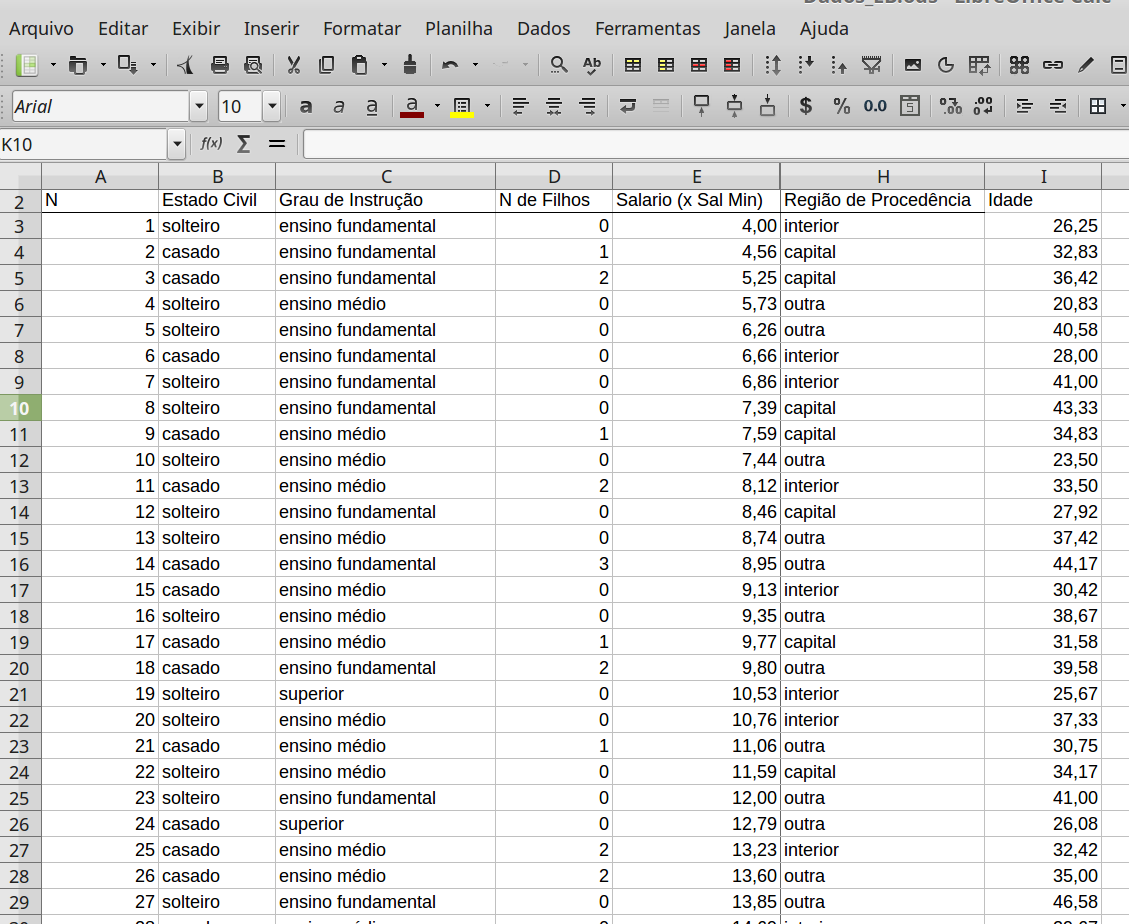
\includegraphics[width = 9cm]{tabela21.png}
\end{figure}
\end{frame}

\section{Variável Qualitativa (Nominal ou Ordinal)}

\begin{frame}{}
	\begin{block}{Tabela de distribuição de frequência}
		Contagem do número de vezes que um valor possível aparece na amostra.
	\end{block}
	
	\begin{table}
		\centering
		\begin{tabular}{l|ccc}
			\toprule[0.05cm]
			Variável & Frequência & Frequência Relativa & Porcentagem \\ \midrule[0.05cm]
			categoria 1 & $n_1$ & $f_1=\frac{n_1}{n}$ & $100 \cdot f_1 \%$\\
			categoria 2 & $n_2$ & $f_2=\frac{n_2}{n}$ & $100 \cdot f_2\%$\\
			\vdots & \vdots & \vdots & \vdots \\
			categoria k & $n_k$ & $f_k = \frac{n_k}{n}$ & $100 \cdot f_k\%$\\ \midrule[0.05cm]
			Total & $n=n_1 + n_2 + \cdots + n_k$ & $1$ & $100\%$ \\
			\bottomrule[0.05cm]
		\end{tabular}
	\end{table}
	
	\begin{description}
		\item[$n_i$] Número de elementos da população com variável igual a categoria $i, i=1,2, \dots, k$;
		\item[$f_i$] Proporção ou frequência relativa calculada por $f_i = \frac{n_i}{n}, i=1,2,\dots,k$, em que $n=n_1+n_2+\dots+n_k$.
	\end{description}

\end{frame}


\begin{frame}{Exemplo}
	Variável Escolaridade (Y).
	\begin{table}
		\centering
		\begin{tabular}{l|ccc}
			\toprule[0.05cm]
			Y  & Frequência & Frequência Relativa & Porcentagem\\ \midrule[0.05cm]
			Ensino Fundamental & $12$ & $0,3333$ & $33,33\%$\\ 
			Ensino Médio & $18$ & $0,5$ & $50\%$ \\
			Ensino Superior & $6$ & $0,1667$ & $16,67\%$ \\
			\midrule[0.05cm]
			Total & $36$ & $1$ & $100\%$\\
			\bottomrule[0.05cm]
		\end{tabular}
	\end{table}
	

\end{frame}

\begin{frame}{Exemplo -- continuação}
	\begin{figure}
	\centering
	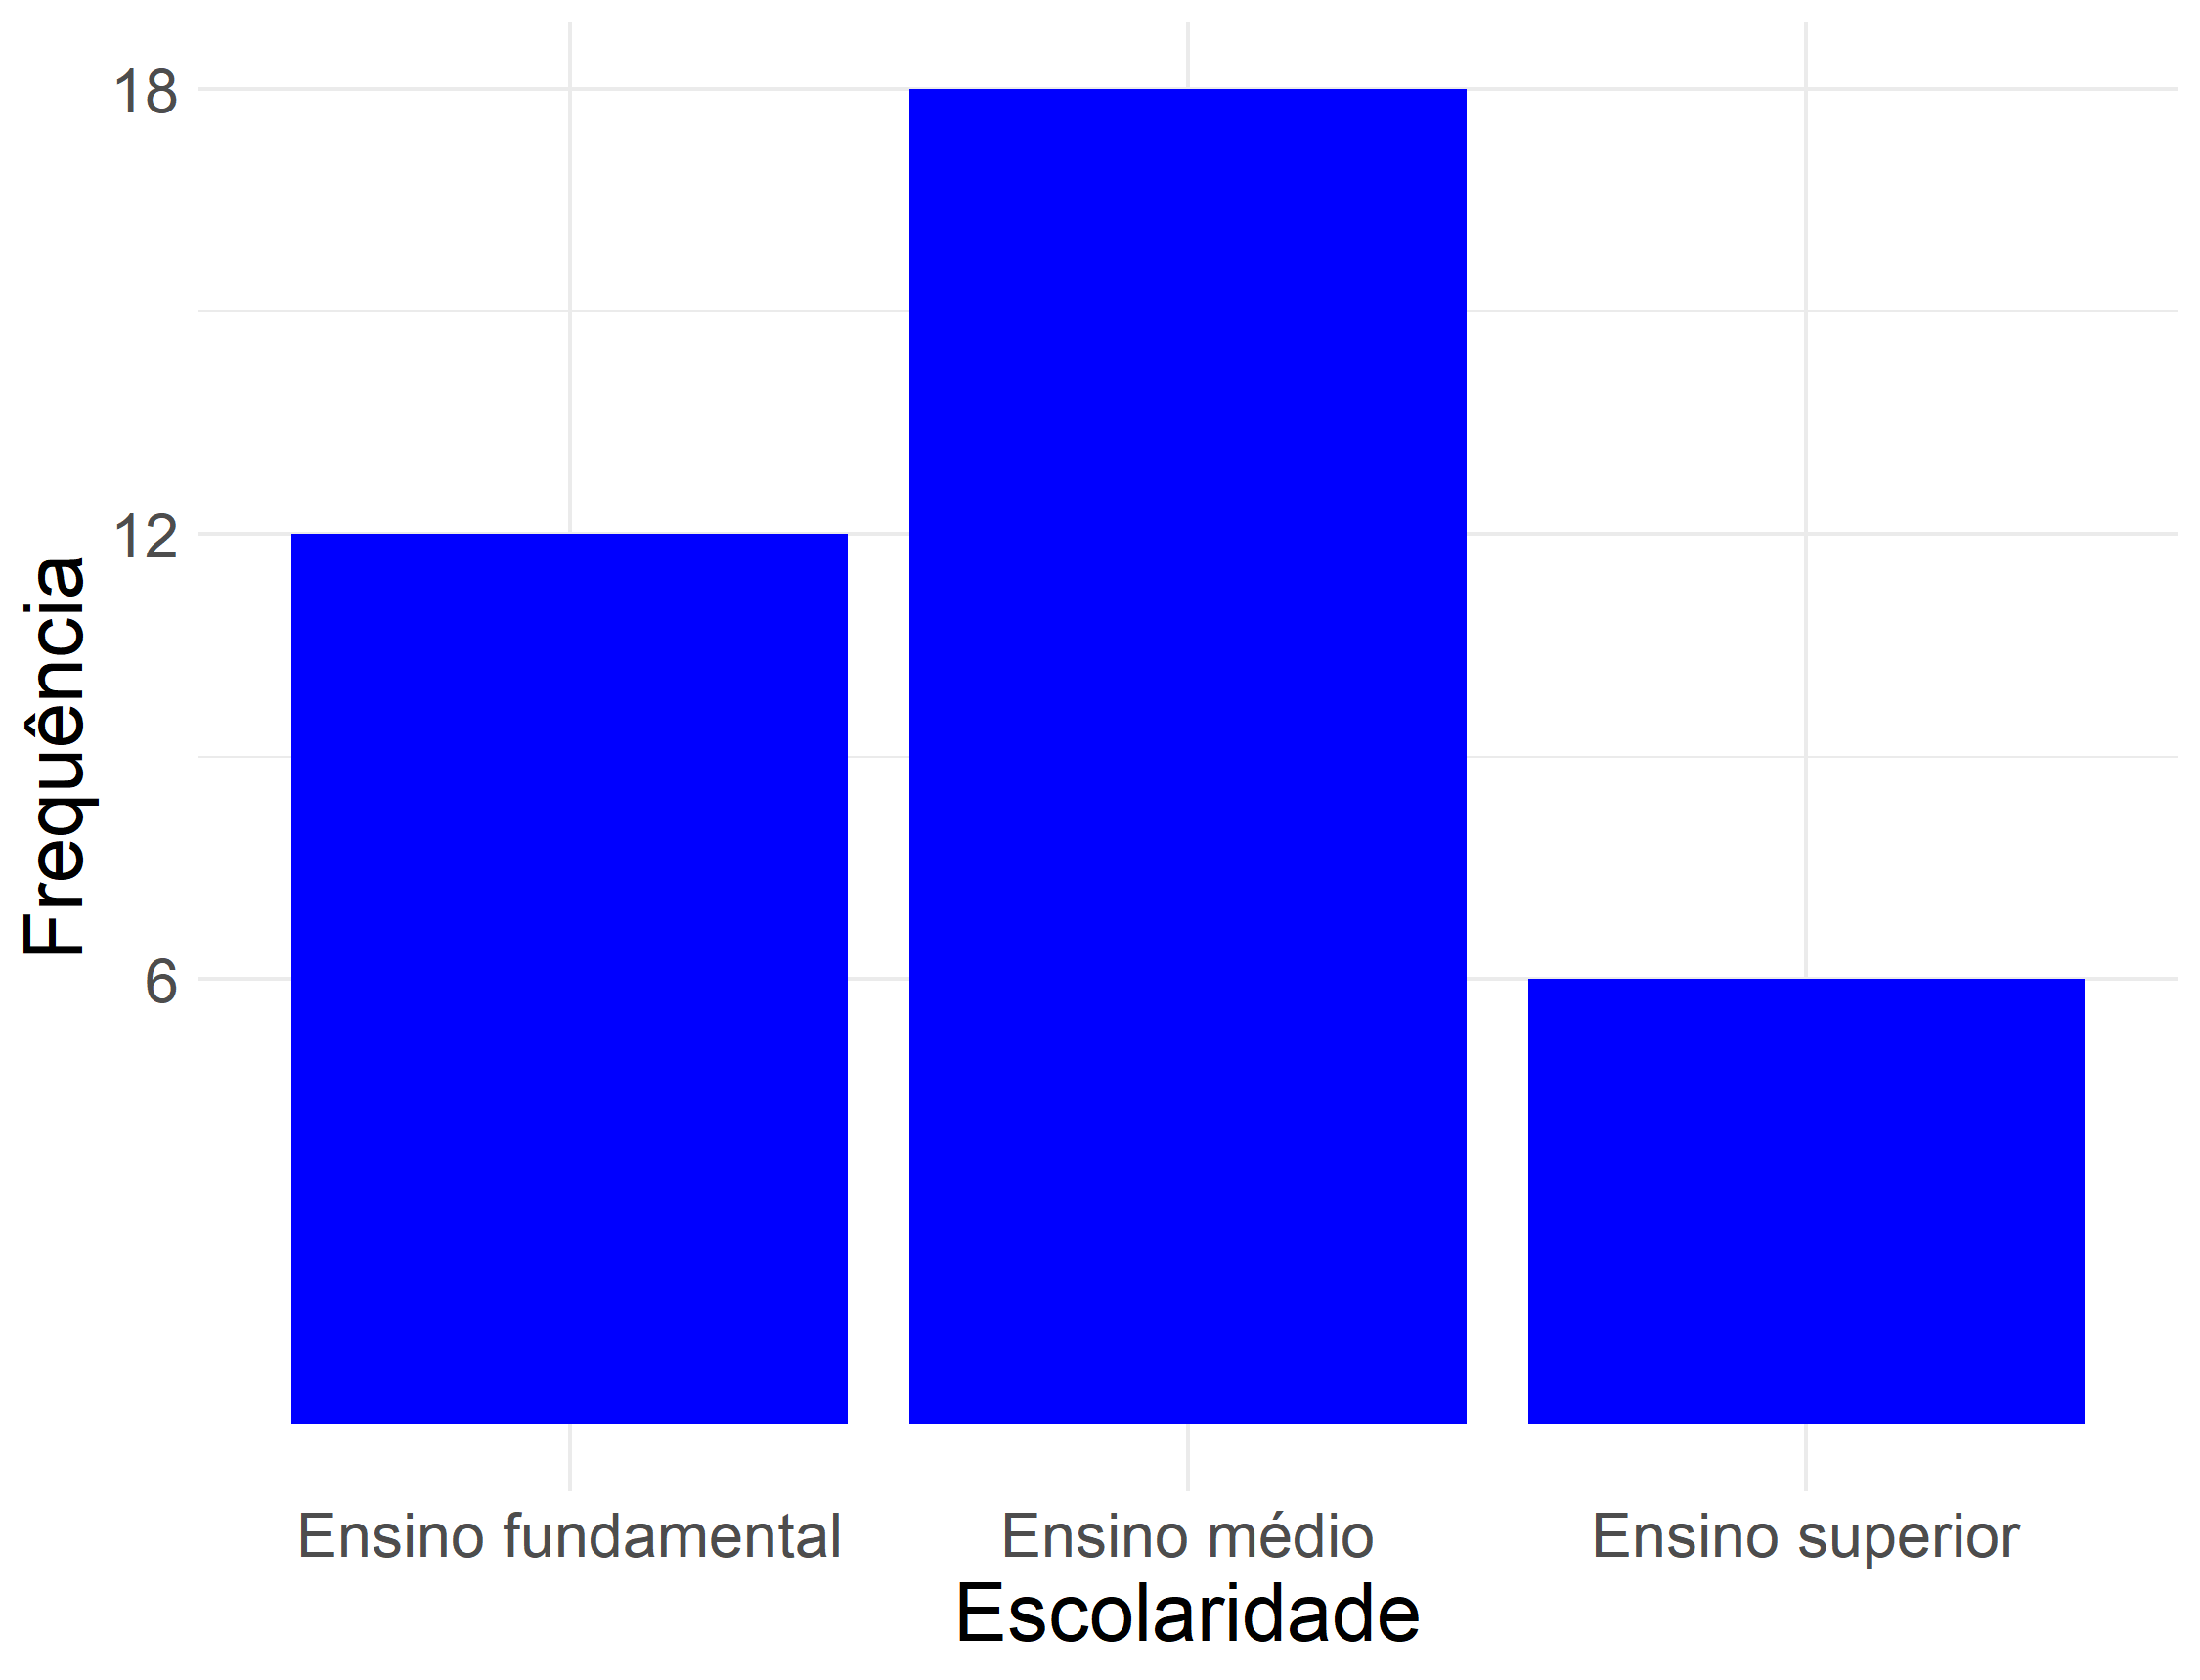
\includegraphics[height=6cm]{escolaridade.png}
\end{figure}
\textbf{Interpretação:} O grau de escolaridade mais presente entre os funcionários é ``Ensino Médio'', podemos inclusive dizer que esse atributo é maioria entre os funcionários da companhia MB.
\end{frame}

\section{Variável Quantitativa Descritiva}

\begin{frame}{Exemplo}
	Número de filhos (Z).
	\begin{table}
		\centering
		\begin{tabular}{l|ccc}
			\toprule[0.05cm]
			Z & Frequência & Frequência relativa & Porcentagem\\ \midrule[0.05cm]
			$0$ & $20$ & $0,5556$ & $55,56\%$\\
			$1$ & $5$ & $0,1386$ & $13,86\%$\\
			$2$ & $7$ & $0,1944$ & $19,44\%$\\
			$3$ & $3$ & $0,0833$ & $8,33\%$\\
			$4$ & $0$ & $0,00$ & $0,00\%$\\
			$5$ & $1$ & $0,0278$ & $2,78\%$\\ \midrule[0.05cm]
			Total & $36$ & $1$ & $100\%$\\ \bottomrule[0.05cm]
		\end{tabular}
	\end{table}
\end{frame}

\begin{frame}{Exemplo -- continuação}
	\begin{figure}
		\centering
		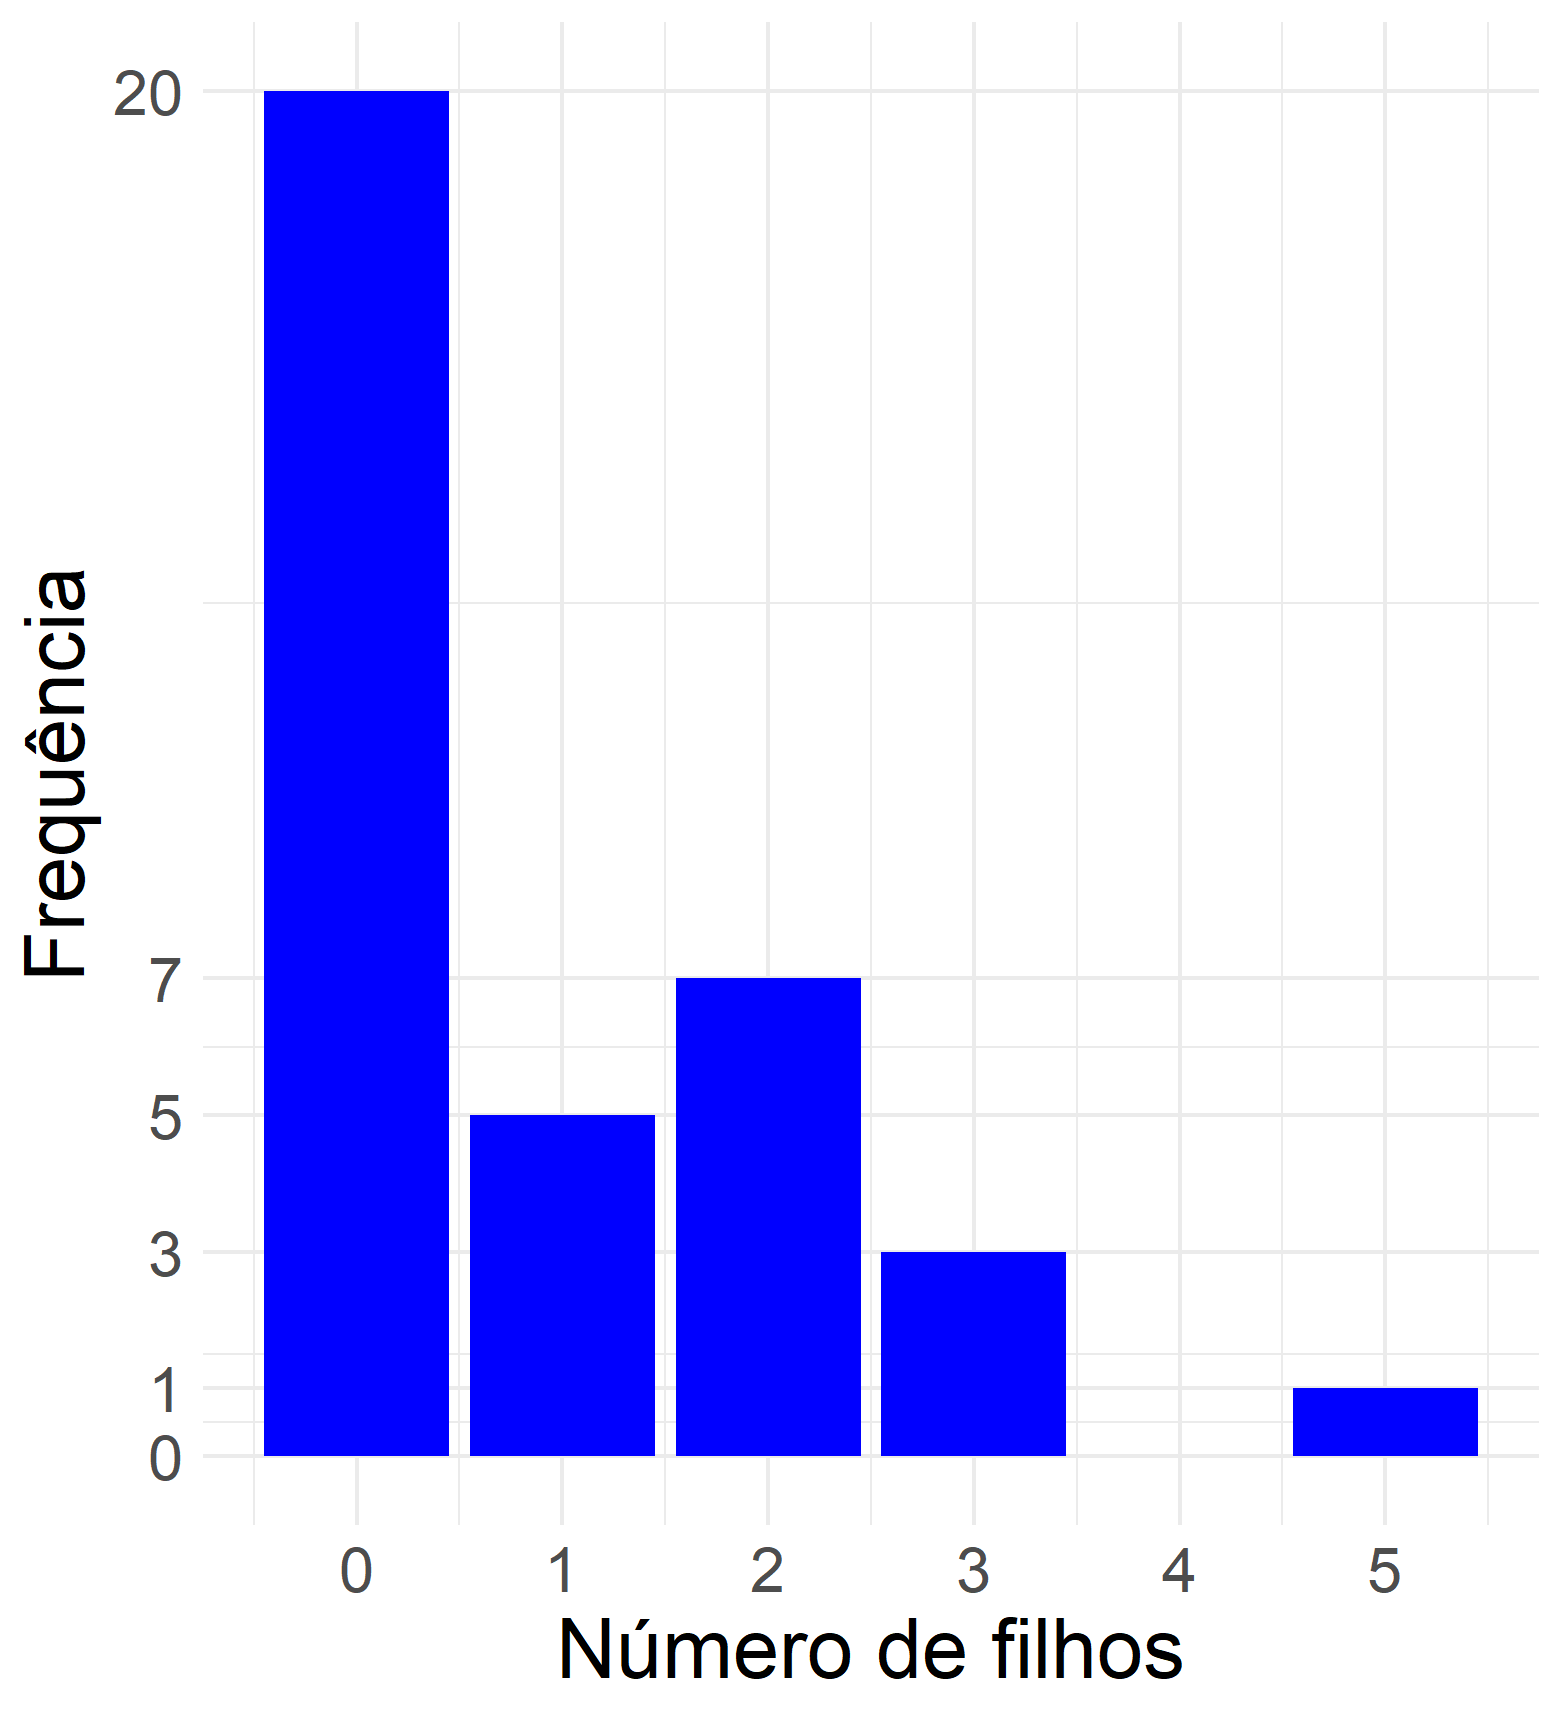
\includegraphics[width = 6cm]{numero_filhos.png}
	\end{figure}
\textbf{Interpretação:} A maioria dos funcionários tem até 2 filhos.
\end{frame}

\section{Variável Quantitativa Contínua}

\begin{frame}{Exemplo}
	Salário (S).
	\begin{table}
		\centering
		\begin{tabular}{l|ccc}
			\toprule[0.05cm]
			S & Frequência & Frequência relativa & Porcentagem\\ \midrule[0.05cm]
			$[4,8)$ & $10$ & $0,2778$ & $27,78\%$\\
			$[8,12)$ & $12$ & $0,3333$ & $33,33\%$\\
			$[12,16)$ & $8$ & $0,2222$ & $22,22\%$\\
			$[16,20)$ & $5$ & $0,1389$ & $13,89\%$\\
			$[20,24]$ & $1$ & $0,0278$ & $2,78\%$\\
			\midrule[0.05cm]
			Total & $36$ & $1$ & $100\%$\\ \bottomrule[0.05cm]
		\end{tabular}
	\end{table}
\end{frame}

\begin{frame}{Exemplo -- continuação}
	\begin{block}{Simplificação}
		Representamos cada faixa da variável contínua pelo seu ``ponto médio''.
	\end{block}
		
	\begin{table}
		\centering
		\begin{tabular}{l|cc}
			\toprule[0.05cm]
			Salário & Ponto Médio & Frequência \\ \midrule[0.05cm]
			$[4,8) $ & 6 & 10\\
			$[8,12) $ & 10 & 12\\
			$[12,16) $ & 14 & 8\\
			$[16,20) $ & 18 & 5\\
			$[20,24] $ & 22 & 1\\
			\bottomrule[0.05cm]
		\end{tabular}
	\end{table}
	\begin{block}{Observação}
	  Em nosso exemplo, estamos afirmando que todos os funcionários da faixa salarial $[4,8)$ ganham aproximadamente $6$ salários mínimos.
	\end{block}

\end{frame}

\begin{frame}{Exemplo -- continuação}
  \begin{figure}
   \centering
   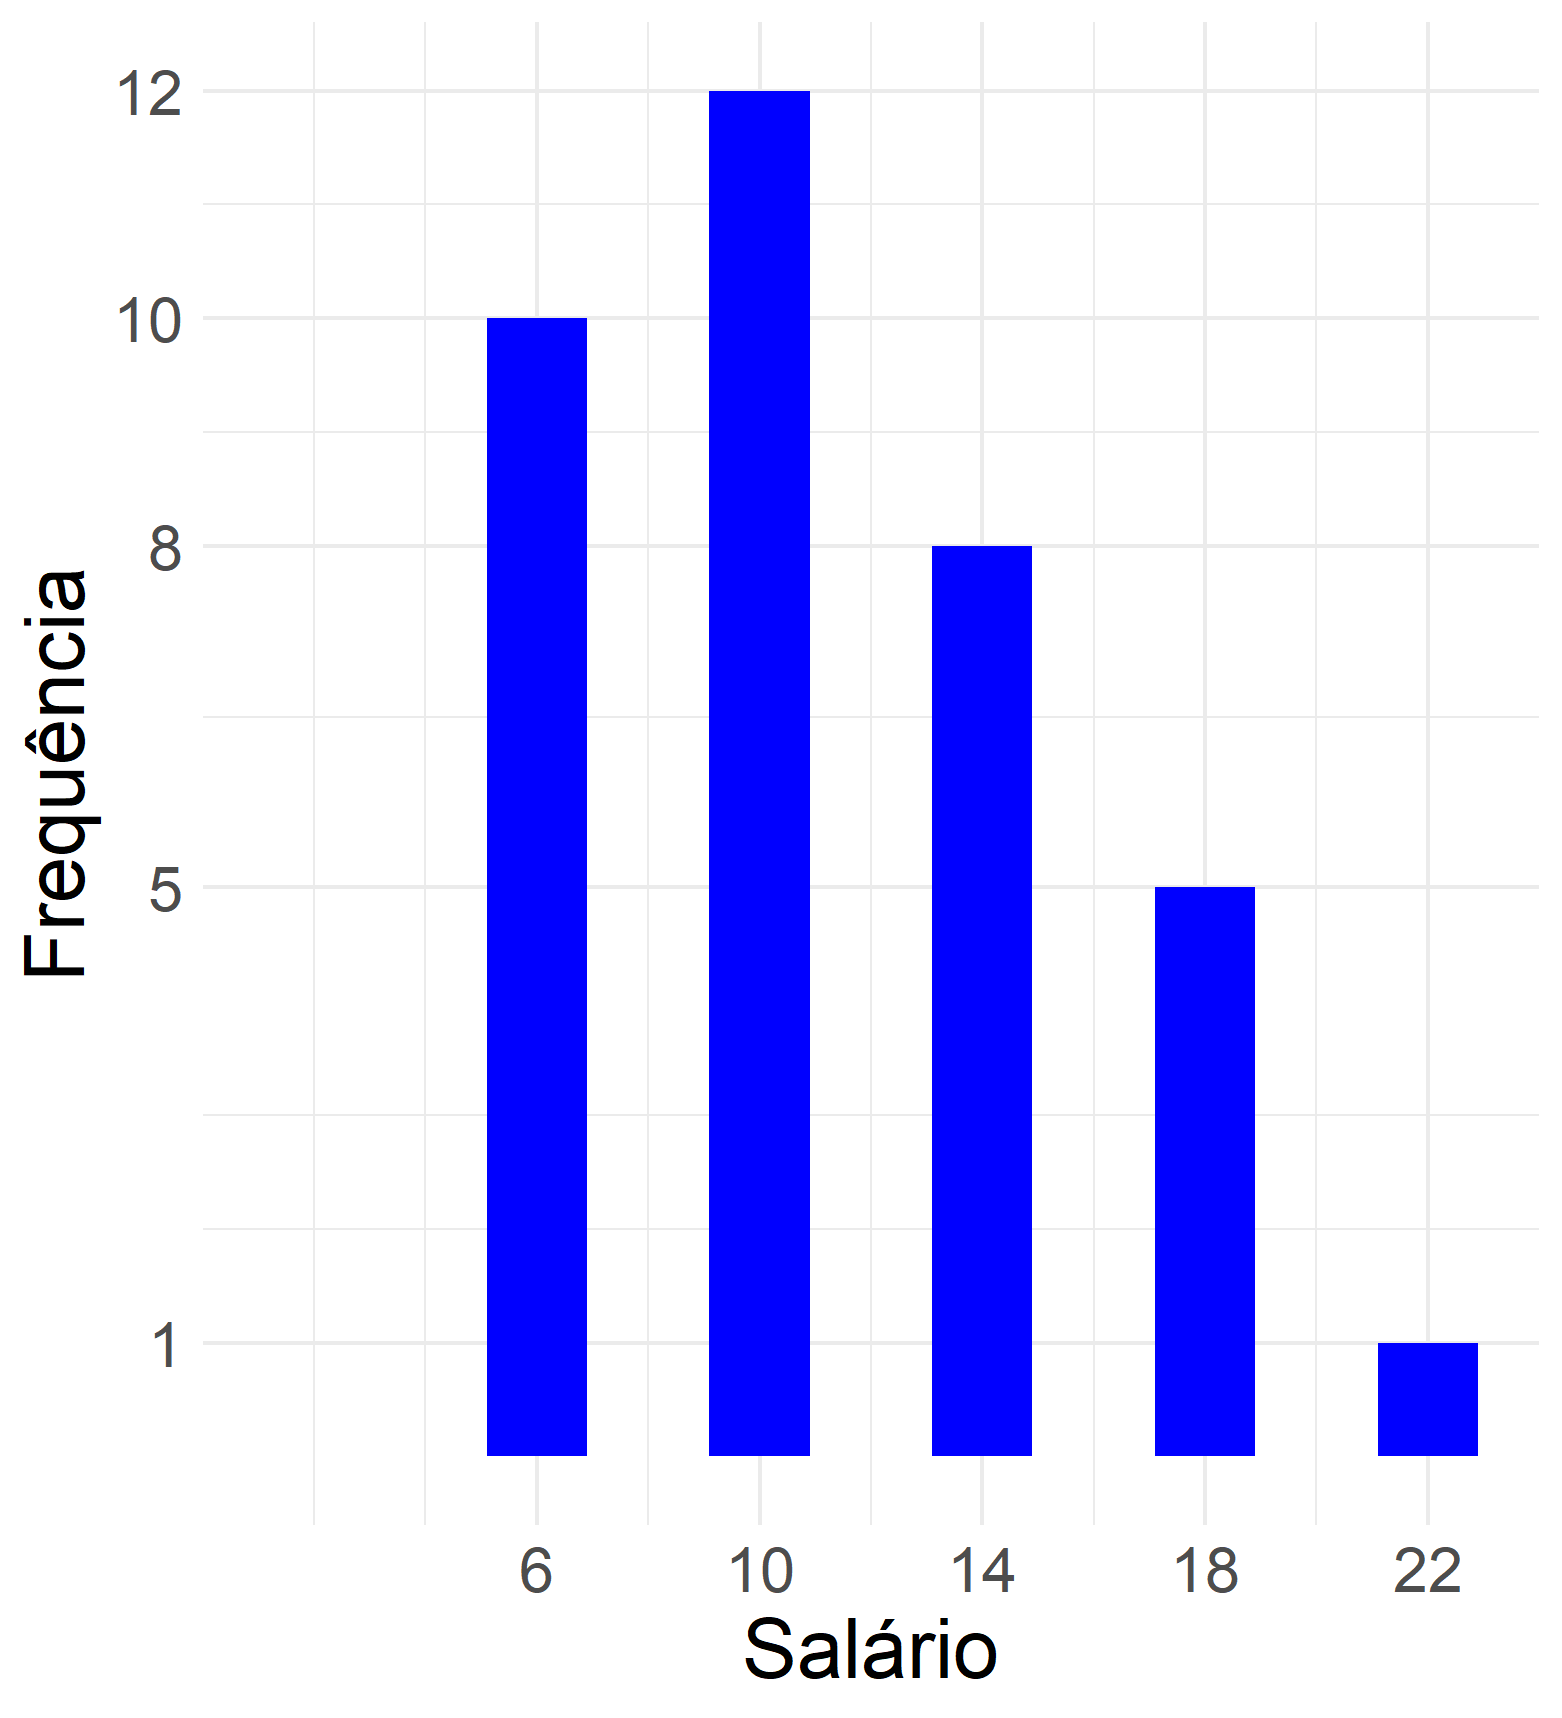
\includegraphics[height=6cm]{salario_bar.png}
  \end{figure}
  
  \textbf{Interpretação:} Notamos que o salário mais frequente é dez salários mínimos.
\end{frame}

\subsection{Histograma}

\begin{frame}{}
 \begin{block}{Definição}
  Gráficos de barras contíguas, com as bases proporcionais a largura das classes/faixas e a área de cada retângulo proporcional à respectiva frequência relativa.
 \end{block}
 
 \begin{block}{Notação}
  \begin{description}
   \item[$\Delta_i:$] amplitude da $i$-ésima barra;
   \item[$\frac{f_i}{\Delta_i}:$] altura da barra chamada de densidade de frequência.
  \end{description}
 \end{block}
 
 \begin{figure}
  \centering
  \begin{tikzpicture}
   \filldraw[blue!30] (1,0) rectangle (3,2);
   \draw[black] (1,0) rectangle (3,2);
   \node at (2,1) {$f_i = \frac{f_i}{\Delta_i}\cdot \Delta_i$};
    \draw[->] (0,0) -- (0,3);
   \draw[->] (0,0) -- (4,0);
   \node[right] at (4,0) {Variável contínua};
   \node[above] at (0,3) {Denside de frequência};
   \draw[decorate,decoration={brace,mirror}] (3,0) -- (3,2);
   \node[right] at (3,1) {$\frac{f_i}{\Delta_i}$}; 
   \draw[decorate,decoration={brace,mirror}] (1,0) -- (3,0);
   \node[below] at (2,0) {$\Delta_i$};
  \end{tikzpicture}

 \end{figure}

\end{frame}

\begin{frame}{Exemplo}
 Salário (S).
 \begin{table}
  \centering
  \begin{tabular}{l|ccc}
   \toprule[0.05cm]
   Salário & Amplitude $(\Delta_i)$ & Frequência $(f_i)$ & Densidade de frequência $\left(\frac{f_i}{\Delta_i}\right)$\\
   \midrule[0.05cm]
    $[4,8)$ & $4$ & $0,2778$ & $\frac{0,2778}{4}=0,0694$\\
    $[8,12)$ & $4$ & $0,3333$ & $\frac{0,3333}{4}=0,0833$\\
    $[12,16)$ & $4$ & $0,2222$ & $\frac{0,2222}{4}=0,0556$\\
    $[16,20)$ & $4$ & $0,1389$ & $\frac{0,1389}{4}=0,0347$\\
    $[20,24]$ & $4$ & $0,0278$ & $\frac{0,0278}{4}=0,0069$\\
    \bottomrule[0.05cm]
  \end{tabular}
 \end{table}

\end{frame}

\begin{frame}{Exemplo -- continuação}
 \begin{figure}
  \centering
  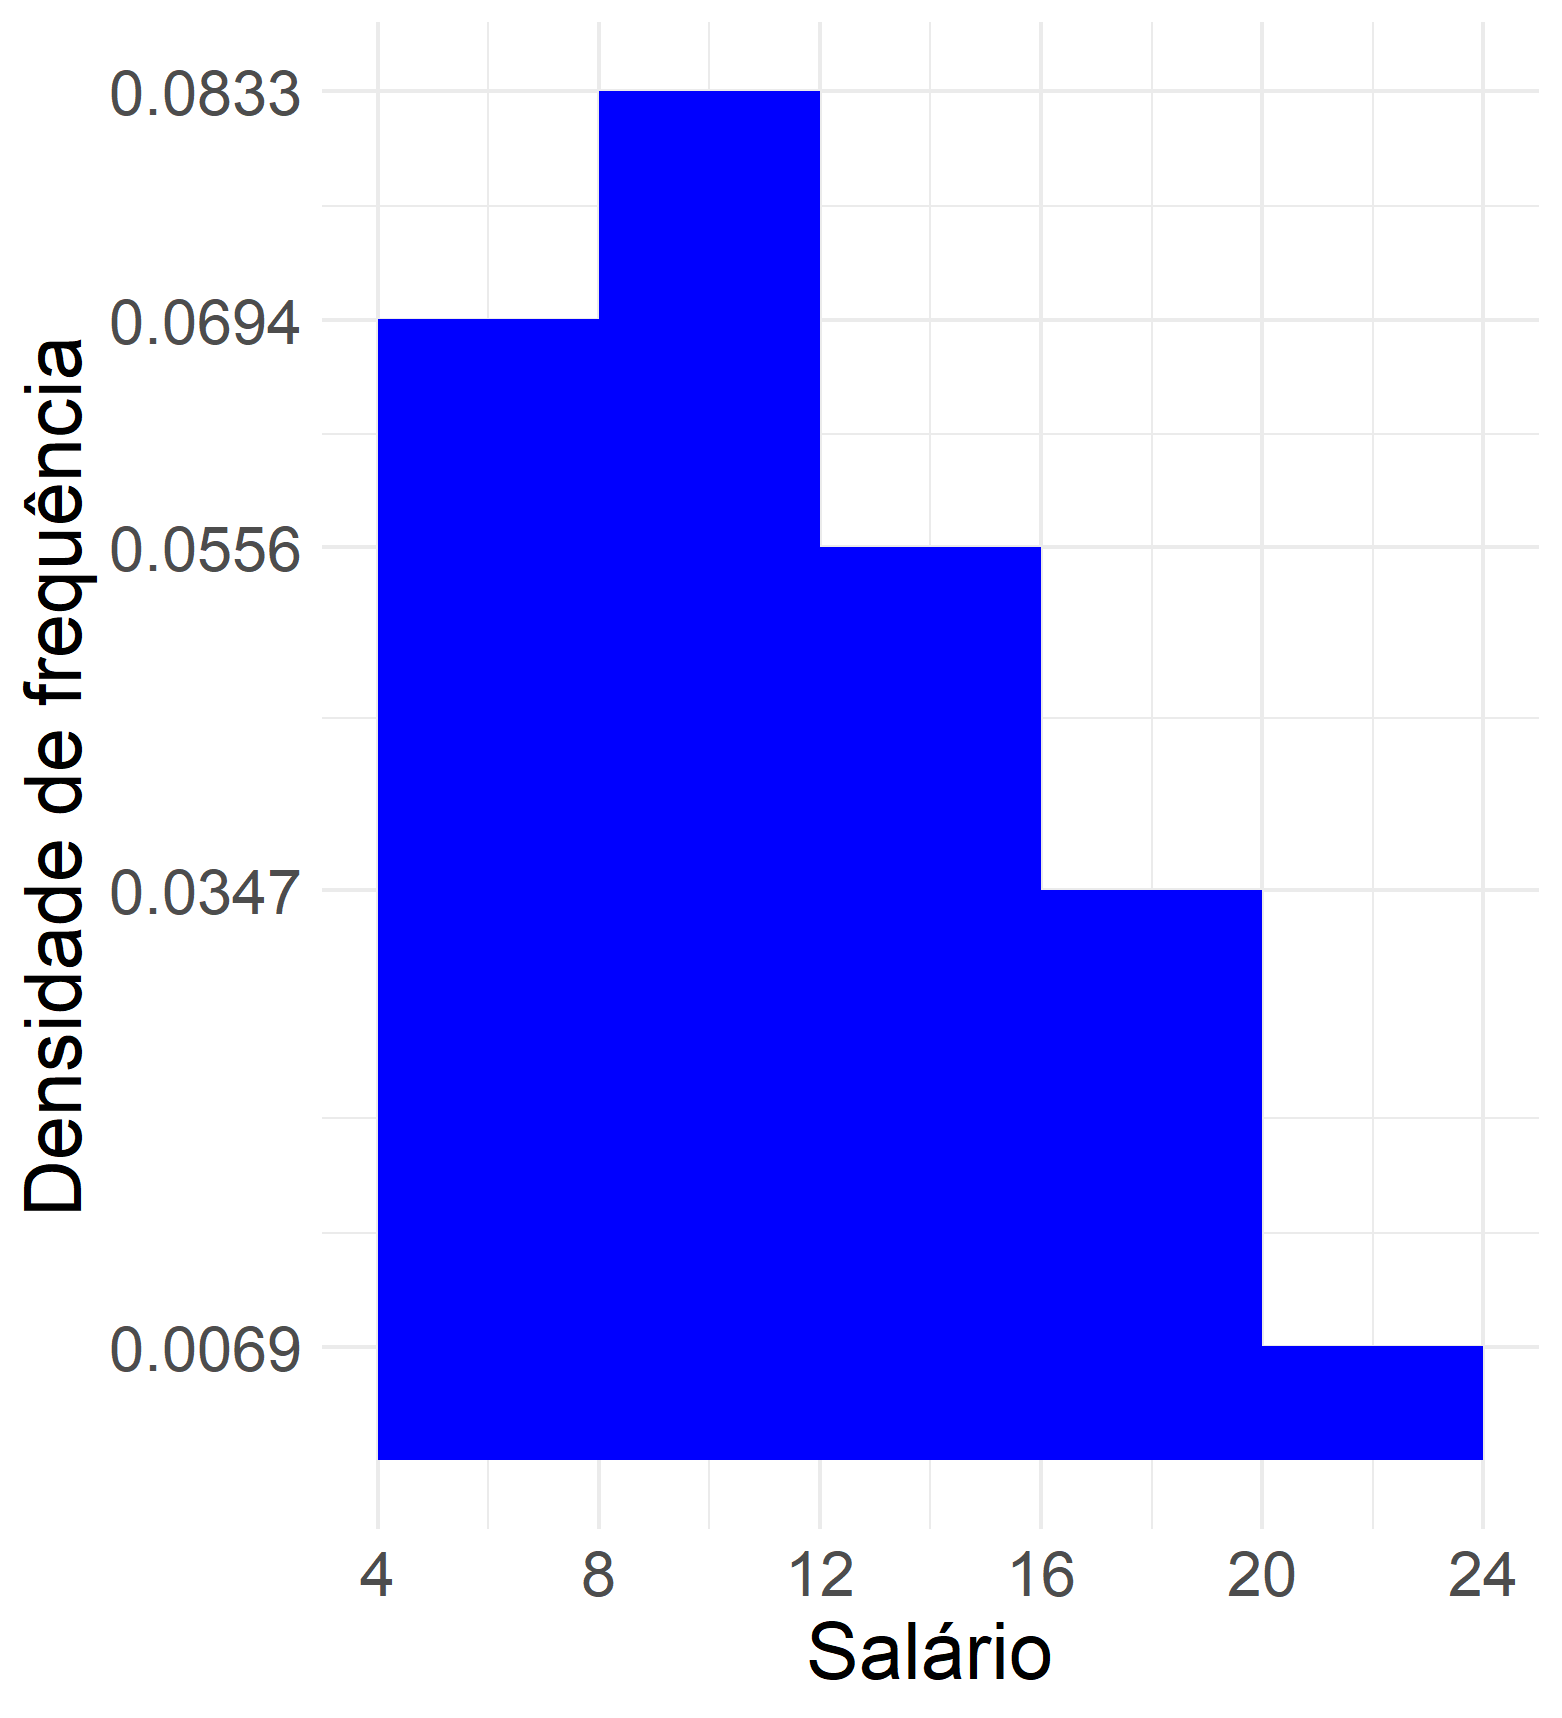
\includegraphics[height=6cm]{histograma.png}
 \end{figure}
\textbf{Interpretação:} A maioria dos funcionários ganham entre 4 e 12 salários mínimos.
\end{frame}

\end{document}